\documentclass[runningheads,a4paper]{llncs}
\usepackage[utf8]{inputenc}
\usepackage[T1]{fontenc}
\usepackage{csquotes}
\usepackage[english]{babel}
\usepackage[backend=bibtex,natbib,hyperref=true,maxnames=2,style=authoryear-comp]{biblatex}
\addbibresource{seminarreport.bib}

\usepackage{amsmath}
\usepackage{booktabs}
\usepackage{enumitem}
\usepackage{graphicx}
\usepackage{eurosym}
\usepackage[hidelinks]{hyperref}
\usepackage[capitalise]{cleveref}

\DeclareMathOperator*{\somefunc}{somefunc}
%
\begin{document}
%
\frontmatter          % for the preliminaries
%
\pagestyle{headings}  % switches on printing of running heads
%
\mainmatter              % start of the contributions
%
\title{Your Topic}
\subtitle{Seminar/Lab Title}
%
\titlerunning{Lab Title (again!)}  % abbreviated title (for running head)
%
\author{Last Name, First Name}
%
\authorrunning{Last name, first name}   % abbreviated author list (for running head)
\institute{Universit\"at Bonn\\
\email{EMAIL@cs.uni-bonn.de},
Matrikelnummer: XXXXXX
}

\maketitle              % typeset the title of the contribution

\begin{abstract}
    This is  the abstract. It summarizes your  contribution. It should only
    have one paragraph, but very briefly summarize everything in your document.
\end{abstract}

\section{Introduction}

Object recognition in real cluttered environments is hard where objects usually touch or occlude each other.
The paper presents a novel approach to solve the problem using geometric based categorization and perceptual grouping.
Geometric based categorization categorizes the different objects according to their general geometric shape (spheres, boxes, flat objects, cylindrical objects, and disks/plates).
Perceptual grouping choose what geometric shapes stick together to form an object.                                                      

\section{Method}
The main idea of the paper is Inspired by the ideas introduced by Biederman [6] (TODO: Say somthing more about it) recognition-by-components: A theory of human image understanding. Psychological Review (1987)

The idea is also supported in Improving Spatial Support for Objects
via Multiple Segmentations
Lai, K., Fox, D.: Object recognition in 3d point clouds using web data and domain
adaptation.  The International Journal of Robotics Research

{ Using Web Catalogs to Locate and Categorize Unknown Furniture Pieces in 3D
Laser Scans.  Robotics & Automation Magazine
18

7.  Malisiewicz, T., Efros, A.A.:  Improving Spatial Support for Objects via Multiple
Segmentations.  In: Proceedings of the British Machine Vision Conference. (2007)


In paper 29
If the feature is additive, the descriptor that would be computed for the object is
the same as the sum of the features of its segments

There are of course multiple ways of combining segments and not all of them
create a valid object. However, we can test if a combination is valid by checking if
the combined feature vector is known. We also exploit the fact that segments and
their connections (neighborhood relations) can be treated as a graph, and only
certain types of sub-graphs are present in the graph formed by the parts of an
object. Checking for subgraph isomorphism is not practical, but there are several
descriptors one can employ to rule out isomorphism. Thus, during training we
decompose  our  objects  into  parts,  compute  the  features  for  each  part,  build
the part-graph, and generate all sub-graphs along with their combined features.
Figure 2 shows an overview of the main steps of our method

\section{Steps}
\begin{enumerate}
    \item Object categorization
    \item Build graph for each part
    \item Selection of Geometry-Based Categories
    \item Calculate arrangement keys
\end{enumerate}

\section{Feature detector}


\subsection{RSD}
Encodes the radial relationship of the point and its neighborhood. 
For every pair of the keypoint with a neighbor, computes the distance between them and the difference between their normals. 
Find a sphere that fits the points and their normals.
From all the point-neighbor spheres, only the ones with the maximum and minimum radii are kept and saved to the descriptor of that point. 

When two points lie on a flat surface, the sphere radius will be infinite. 
If they lie on the curved face of a cylinder, the radius will be more or less the same as that of the cylinder. 
This allows us to tell objects apart with RSD. The algorithm takes a parameter that sets the maximum radius at which the points will be considered to be part of a plane.


\subsection{GRSD}
GRSD is a histogram that counts the number of transitions between different types of voxels (Sphere, box, rectangle, cylindrical, plate).

\begin{figure}[!htbp]
    \centering
    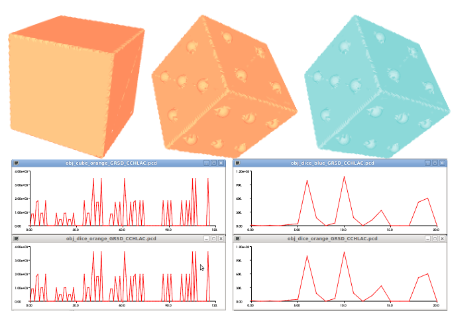
\includegraphics[width=0.5\linewidth]{pic/rsd.png}
    \caption{Rotation-invariant  C 3 -HLAC  can  not  differentiate the  die  from  the  cube  (identical  histograms  on  the  left), while GRSD/GRSD 2 can not differentiate the different colors (identical histograms on the right). Their combination how- ever produces distinct signatures for all of them. Photo courtesy: \citep{Marton2012} }
    \label{fig::photo_nuts}    
\end{figure}

\subsection{GRSD-}
adapted the GRSD feature to be additive, by simplifying it to simple histogram of neighborhoods of surfaces of dierent type, neglecting the ray-tracing step

\subsection{C³-HLAC}



\section{Conclusion}

\printbibliography
\end{document}
